\chapter{Computational Study}

This chapter presents our computational study and is structured as follows: Section 5.1 describes the data our experiments are conducted on.  
\section{Data description}

The available data set is provided by \cite{Hildebrandt2020_EAT} who created a high-dimensional data model with the RMDP instances originally used in \cite{UlmerRMDP}. It comprises 850.469 samples, 23.341 unique customer locations, a delivery fleet of 15 vehicles and 15 unique restaurant locations. The temporal and spatial distribution of the orders is depicted in figure \ref{fig:dists}. 
\begin{figure}[h]
	\centering
	\subfigure[Request arrival time distribution]{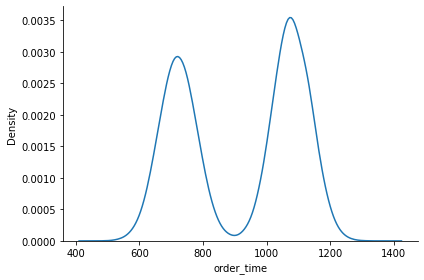
\includegraphics[width=0.49\linewidth]{../Implementation/Plots/order_time_dist.png}}
	\subfigure[Spatial distributions]{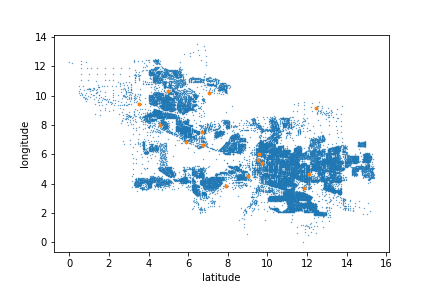
\includegraphics[width=0.49\linewidth]{../Implementation/Plots/spatial_dist.png}}
	\caption{Spatial and temporal distributions}
	\label{fig:dists}
\end{figure}

Panel (a) of figure \ref{fig:dists} shows the order behaviour of customers. The x-axis denotes the day time in minutes, the y-axis denotes the relative frequency of incoming customer orders for a given day time on the y-axis. We can observe that the order time behaviour across all customers follows a bimodal gaussian distribution. The order frequency peaks at around 12:00 a.m (roughly 700 minutes of day time) and again around 6.00 p.m (roughly 1100 minutes of day time). This indicates that the probability of an order taking place during lunch or dinner time is relatively high.  
Panel (b) of figure \ref{fig:prepdelay} 
\begin{figure}[h]
	\centering
	\subfigure[]{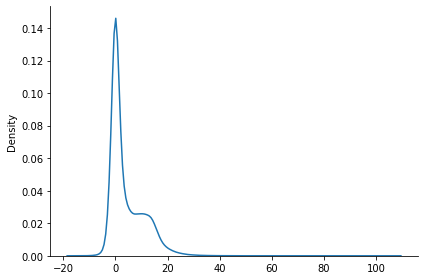
\includegraphics[width=0.49\linewidth]{../Implementation/Plots/delivery_delay.png}}
	\subfigure[Temporal distributions]{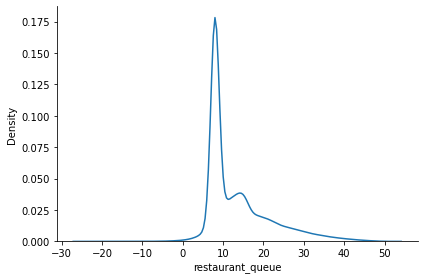
\includegraphics[width=0.49\linewidth]{../Implementation/Plots/prep_time.png}}
	\caption{Spatial and temporal distributions}
	\label{fig:prepdelay}
\end{figure}
 
\section{Parametrization of Methods}

\section{Results}







